\documentclass[sigconf]{acmart}

\usepackage{booktabs} % For formal tables
\usepackage[utf8]{inputenc}

% Copyright
%\setcopyright{none}
%\setcopyright{acmcopyright}
%\setcopyright{acmlicensed}
\setcopyright{rightsretained}
%\setcopyright{usgov}
%\setcopyright{usgovmixed}
%\setcopyright{cagov}
%\setcopyright{cagovmixed}


% DOI
\acmDOI{xxxxxxx}

% ISBN
\acmISBN{xxxxxx}

%Conference
\acmConference[SBSI'19]{Simpósio Brasileiro de Sistemas de Informação}{Maio 2019}{Aracaju/SE - Brasil}
\acmYear{2019}
\copyrightyear{2019}


\acmArticle{4}
\acmPrice{15.00}


\begin{document}
\title{Utilizando Ontologias para apoiar a recomendação de revisores de código entre projetos distintos}

\author{Vinicius J. Schettino}
\affiliation{%
\institution{Universidade Federal de Juiz de Fora}
  \streetaddress{}
  \city{Juiz de Fora}
  \state{Minas Gerais}
}
\email{vinicius.schettino@ice.ufjf.br}

\author{Regina Braga}
\affiliation{%
  \institution{Universidade Federal de Juiz de Fora}
  \streetaddress{}
  \city{Juiz de Fora}
  \state{Minas Gerais}
}\email{regina.braga@ufjf.edu.br}

\author{Marco Antônio P. Araújo}
\affiliation{%
  \institution{Universidade Federal de Juiz de Fora}
  \streetaddress{}
  \city{Juiz de Fora}
  \state{Minas Gerais}
}\email{marco.araujo@ufjf.edu.br}

\author{Victor Ströele}
\affiliation{%
  \institution{Universidade Federal de Juiz de Fora}
  \streetaddress{}
  \city{Juiz de Fora}
  \state{Minas Gerais}
}\email{victor.stroele@ufjf.edu.br}

% The default list of authors is too long for headers.
\renewcommand{\shortauthors}{Schettino et al.}


\begin{abstract}
A prática de \textit{code review} está amplamente associada a qualidade de código e detecção precoce de defeitos de software. Intrinsecamente colaborativo, a eficiência do processo depende também do perfil histórico do revisor e da natureza do código em avaliação. Em contexto de desenvolvimento distribuído, consolidar todas as informações que ajudam a encontrar o revisor adequado se torna ainda mais difícil, e a importância da recomendação automatizada ganha mais força. Dentre outros desafios, a arquitetura e habilidades necessárias entre projetos são distintas, atrapalhando a troca de experiências e auxílios entre diferentes grupos de trabalho. Para auxiliar no processo de escolha do revisor, uma ontologia de alinhamento é proposta, de forma a relacionar os tópicos de conhecimento entre projetos distintos. Assim é possível encontrar especialistas que possam ser revisores adequados em diferentes grupos de tabalho. Este estudo apresenta a  arquitetura responsável pela extração dos dados e aplicação da ontologia proposta, exemplificado por um cenário envolvendo projetos OpenSource conhecidos de uma mesma organização.
\end{abstract}

%
% The code below should be generated by the tool at
% http://dl.acm.org/ccs.cfm
% Please copy and paste the code instead of the example below.
%

\begin{CCSXML}
<ccs2012>
<concept>
<concept_id>10011007.10011074.10011134.10003559</concept_id>
<concept_desc>Software and its engineering~Open source model</concept_desc>
<concept_significance>500</concept_significance>
</concept>
<concept>
<concept_id>10011007.10011074.10011134.10011135</concept_id>
<concept_desc>Software and its engineering~Programming teams</concept_desc>
<concept_significance>500</concept_significance>
</concept>
<concept>
<concept_id>10011007.10010940.10010992.10010998.10010999</concept_id>
<concept_desc>Software and its engineering~Software verification</concept_desc>
<concept_significance>300</concept_significance>
</concept>
<concept>
<concept_id>10011007.10011074.10011075.10011077</concept_id>
<concept_desc>Software and its engineering~Software design engineering</concept_desc>
<concept_significance>300</concept_significance>
</concept>
</ccs2012>
\end{CCSXML}

\ccsdesc[500]{Software and its engineering~Open source model}
\ccsdesc[500]{Software and its engineering~Programming teams}
\ccsdesc[300]{Software and its engineering~Software verification}
\ccsdesc[300]{Software and its engineering~Software design engineering}

\keywords{code review, ontology, distributed software development}


\maketitle

\section{Introdução}

O \textit{code review} é considerado uma das principais técnicas para diminuição de defeitos de software \cite{Boehm2001}. O autor de uma alteração na base de código de um projeto submete tal conteúdo ao crivo de um conjunto de pares técnicos, que irão revisar sua estrutura com base em um lista de regras e convenções previamente definidas. Diferentes aspectos relacionados ao autor, ao revisor e ao processo de revisão em si estão diretamente relacionados à eficiência da prática. Autores relatam a diminuição da incidência de \textit{anti-patterns} \cite{Kemerer2009} de acordo com o nível de participação dos envolvidos e cobertura do código revisado \cite{Meneely201437, Morales2015171, Bavota201581}. Reputação \cite{Baysal2013122, Bosu2014} e experiência \cite{Kononenko2015111} do revisor também parecem impactar nos efeitos do \textit{code review}

Intrinsecamente colaborativa, a atividade de \textit{code review} é exercida com suporte de ferramentas computacionais específicas \cite{Bacchelli2013}, principalmente no desenvolvimento distribuído. No contexto de workflows de trabalho descentralizados \cite{gousios2016}, a prática funciona como um \textit{gateway} de qualidade que busca garantir que apenas alterações aderentes aos padrões de qualidade do projeto serão incorporadas à codebase principal. Esta etapa do desenvolvimento se torna uma oportunidade para disseminação de conhecimento, embate de ideias e discussão de melhores práticas entre profissionais de experiência e visões diferentes. Para tanto, percebe-se a necessidade de suporte computacional para essas atividades colaborativas.

Tais aspectos configuram o Desenvolvimento Distribuído de Software (DDS) \cite{herbsleb2003}, onde equipes de desenvolvimento se encontram espalhadas por organizações e espaços geográficos distintos. Esta abordagem vem modificando a relação entre empresas e sistemas, principalmente em relação às estratégias de negócios \cite{audy2007}. As próprias relações de negócios fomentam a distribuição das equipes, procurando diminuição dos custos e a incorporação de mão de obra qualificada que pode estar em qualquer lugar do planeta.


O Desenvolvimento Distribuído de Software afeta o \textit{code review} de duas formas distintas. Primeiro, o processo de revisão pode se tornar lento e ineficiente quando a colaboração é afetada, devido aos baixos níveis de participação e cobertura. O mesmo vale para a disseminação do conhecimento, que fica prejudicada. Outro desafio que se consolida é a escolha do revisor adequado para aquele \textit{patch}. Com um vasto número de opções e pouca informação disponível sobre os aspectos técnicos e gerenciais (e.g. tempo disponível) já que não há contato co-localizado entre eles, a natureza distribuída deste tipo de desenvolvimento dificulta o processo de escolha do revisor, impactando negativamente a eficiência do processo.

 Existem alguns trabalhos que demonstram métodos de recomendação de revisores \cite{yu2014,Xia2015261,jiang2017}. Também foram revisadas outros trabalhos que apontam características de revisões, revisores e autores que possivelmente potencializam a colaboração \cite{Kemerer2009,Bird2015191,Baysal2013122}. Além disso, o desafio de se encontrar potenciais colaboradores se extende para outras áreas, como recomendação de parceiros de pesquisa~\cite{digiampietri2015}.

No contexto de DDS, porém, os os desafios à colaboração co-localizada são potencializados e as soluções tradicionais não são suficientes para fomentar este aspecto das atividades distribuídas \cite{nicolaci2011}. Casey \cite{casey2010} mostra que, com a distribuição geográfica dos times, diversos outros desafios, antes considerados colaterais ou resolvidos, emergem de forma a ameaçar a colaboração entre os membros da equipe: barreiras culturais, temporais e geográficas; reengenharia dos processos de desenvolvimento; resistência em compartilhar informações e conhecimento com os pares distribuídos; entre outros desafios \cite{pimentel2008, silva2009}. Estes utilizam dados de expertise e reputação dos desenvolvedores para apontar os mais adequados para determinado conhecimento. São utilizados dados de proximidade de código ou de semântica com as revisões anteriores. Abordagens mais recentes de recomendação de revisores envolvem informações de colaboração, como por exemplo impacto do trabalho entre um revisor/autor no passado. Estas relações são geralmente modeladas como redes de colaboração e construídas através de análises semânticas de similaridade e frequência de colaboração entre determinados atores. Fu et al. \cite{fu2017} descreve uma recomendação baseada num grafo de relacionamento entre desenvolvedores e seu status de trabalho no projeto. Xia et al. \cite{xia2017} agrupa desenvolvedores utilizando métodos de proximidade para capturar relações implícitas e explícitas. Yu et al. \cite{yu2014,yu2014-2} estendem essa abordagem com métodos de aprendizado de máquina minerando os comentários para extrair metadados e enriquecer o modelo da rede colaborativa. Yang et al. \cite{yang2016} utilizam social network analysis (SNA) baseadas em informações de atividade recente dos potenciais revisores no projeto.

Contudo, é comum que tecnologias como linguagens, bibliotecas e frameworks sejam utilizados em projetos diferentes, fazendo com que a expertise de um desenvolvedor construída em um projeto o faça um potencial revisor adequado para contribuir em outros componentes. Os trabalhos em geral não focam neste tipo de recomendação entre projetos distintos.

Este tipo de auxílio se faz importante dentro de organizações maiores. É o caso, por exemplo, da Apache Foundation \cite{chelkowski2016}, com dezenas de projetos com diferentes linguagens, arquiteturas e propósitos. É possível que desenvolvedores que trabalham em projetos específicos tenham conheciementos aplicáveis em projetos distintos, apesar de sempre ter contribuído em apenas um deles. A quantidade de projetos, desenvolvedores e de características intrínsecas de cada um destes é uma barreira para detecção e recomendação de especialistas entre repositórios distintos.

Existem diversos trabalhos que visam recomendar revisores, alguns já citados em seções anteriores deste texto \cite{yu2014,yu2014-2,Xia2015261,jiang2017,fu2017,xia2017,yang2016}. O foco desta seção é apresentar trabalhos relacionados a recomendação entre projetos distintos e o uso de ontologias para alinhamento de semânticas.

CoRReCT \cite{rahman2016} é uma ferramenta que também utiliza o histórico dos potenciais revisores para predição. Contudo, as informações em questão tangem a história dele como desenvolvedor. O especialista é definido pelas tecnologias com as quais ele trabalhou no passado, definidas como tópicos de conhecimento. A principal inovação da proposta é utilizar o histórico de todas contribuições OpenSource feitas pelo desenvolvedor. A abordagem é similar ao proposto por Mo et al. \cite{mo2015}. A principal inovação da proposta aqui descrita é o uso de ontologias para recomendar especialistas entre projetos distintos. A utilização de ontolgias para recomendação é uma técnica já explorada em trabalhos anteriores~\cite{middleton2001,middleton2004} e indicada como sugestão para trabalhos futuros~\cite{adomavicius2005}, e por isso é um potencial caminho para otimização dos resultados da recomendação.

Uma ontologia pode ser definida como um vocabulário ou linguagem comum para representar conhecimentos \cite{guarino1998}. Para computação, pode ser vista como uma especificação formal, explícita e não ambígua de um conceito compartilhado por diferentes agentes.

Sob o ponto de vista operacional, uma ontologia é composta por: Definições de classes; Relações e Funções. Se tornaram comuns para representação de conhecimento na Web Semântica \cite{berners2001}. As especificações da ontologia permitem a utilização de máquinas de inferências para descoberta de conhecimentos, antes não explícitos, nas informações disponíveis. Estas máquinas inferem propriedades e relacionamentos baseadas em conhecimentos diretamente representados \cite{berners2001}. Assim, no contexto deste trabalho as ontologias serão utilizadas para descrever a relação entre tópicos de conhecimento de projetos distintos, explorando desta forma o potencial de extração de conhecimento implícito trazido pelas ontologias para melhoria da recomendação em code review no contexto de DDS.

Considerando a prática de revisão de código, o uso de ferramentas computacionais se tornou prática comum neste contexto nos últimos anos \cite{Bacchelli2013}. O GitHub é uma plataforma rica em repositórios de projetos de software. Muitos são de código aberto, disponíveis para mineração. São 24 milhões de usuários, 67 milhões de projetos e 47 milhões de revisões\footnote{https://octoverse.github.com/}, também chamadas de \textit{pull requests} no modelo de desenvolvimento ``\textit{pull based}'' \cite{gousios2014}.

Esta característica permite a extração e análise automatizadas das informações sobre as revisões em projetos de código aberto, através de APIs disponibilizadas para este fim. Desta forma, a partir deste repositório, realizamos a extração de métricas, apontadas como relevante para nossos objetivos pela literatura relacionada.

Assim, o objetivo deste estudo é extender a utilização de técnicas de recomendação de revisores para atender demandas entre projetos distintos. Esta extração é baseada em tópicos de conhecimento e na especialidade dos desenvolvedores. A abordagem pode ser vista como um indicador de "projetos sugeridos" para desenvolvedores que buscam novos repositórios para contribuir. A proposta é que, através da mineração dos repositórios e do uso de uma ontologia para realizar a equivalência entre os tópicos de conhecimento de projetos distintos, seja possível intercambiar potenciais revisores.

\section{Metodologia}

Para instanciar a abordagem proposta, é necessário extraír os dados presentes no repositório de software, executar as técnicas de recomendação de revisores e descrever as equivalências entre os tópicos de conhecimento presentes em cada um dos projetos envolvidos. Esta seção descreve cada uma destas etapas.

\subsection{Extração dos Dados}

Os dados da análise foram extraídos do GitHub através da API\footnote{https://developer.github.com/v3/} disponibilizada para desenvolvedores estenderem as funcionalidades da plataforma e integrar novos produtos que agreguem valor ao processo de desenvolvimento. A versão estável para integração foi a v3, que implementa o padrão arquitetural RESTful\cite{fielding2002}. Existe a API recém lançada v4\footnote{https://developer.github.com/v4/}, que utiliza da especificação GraphQL para exposição dos serviços. Esta não foi utilizada devido a documentação ainda recente e pela preferência ao padrão REST. A figura~\ref{fig:processo_extracao} mostra o pipeline de extração e estruturação dos dados.

\begin{figure}[!htbp]
 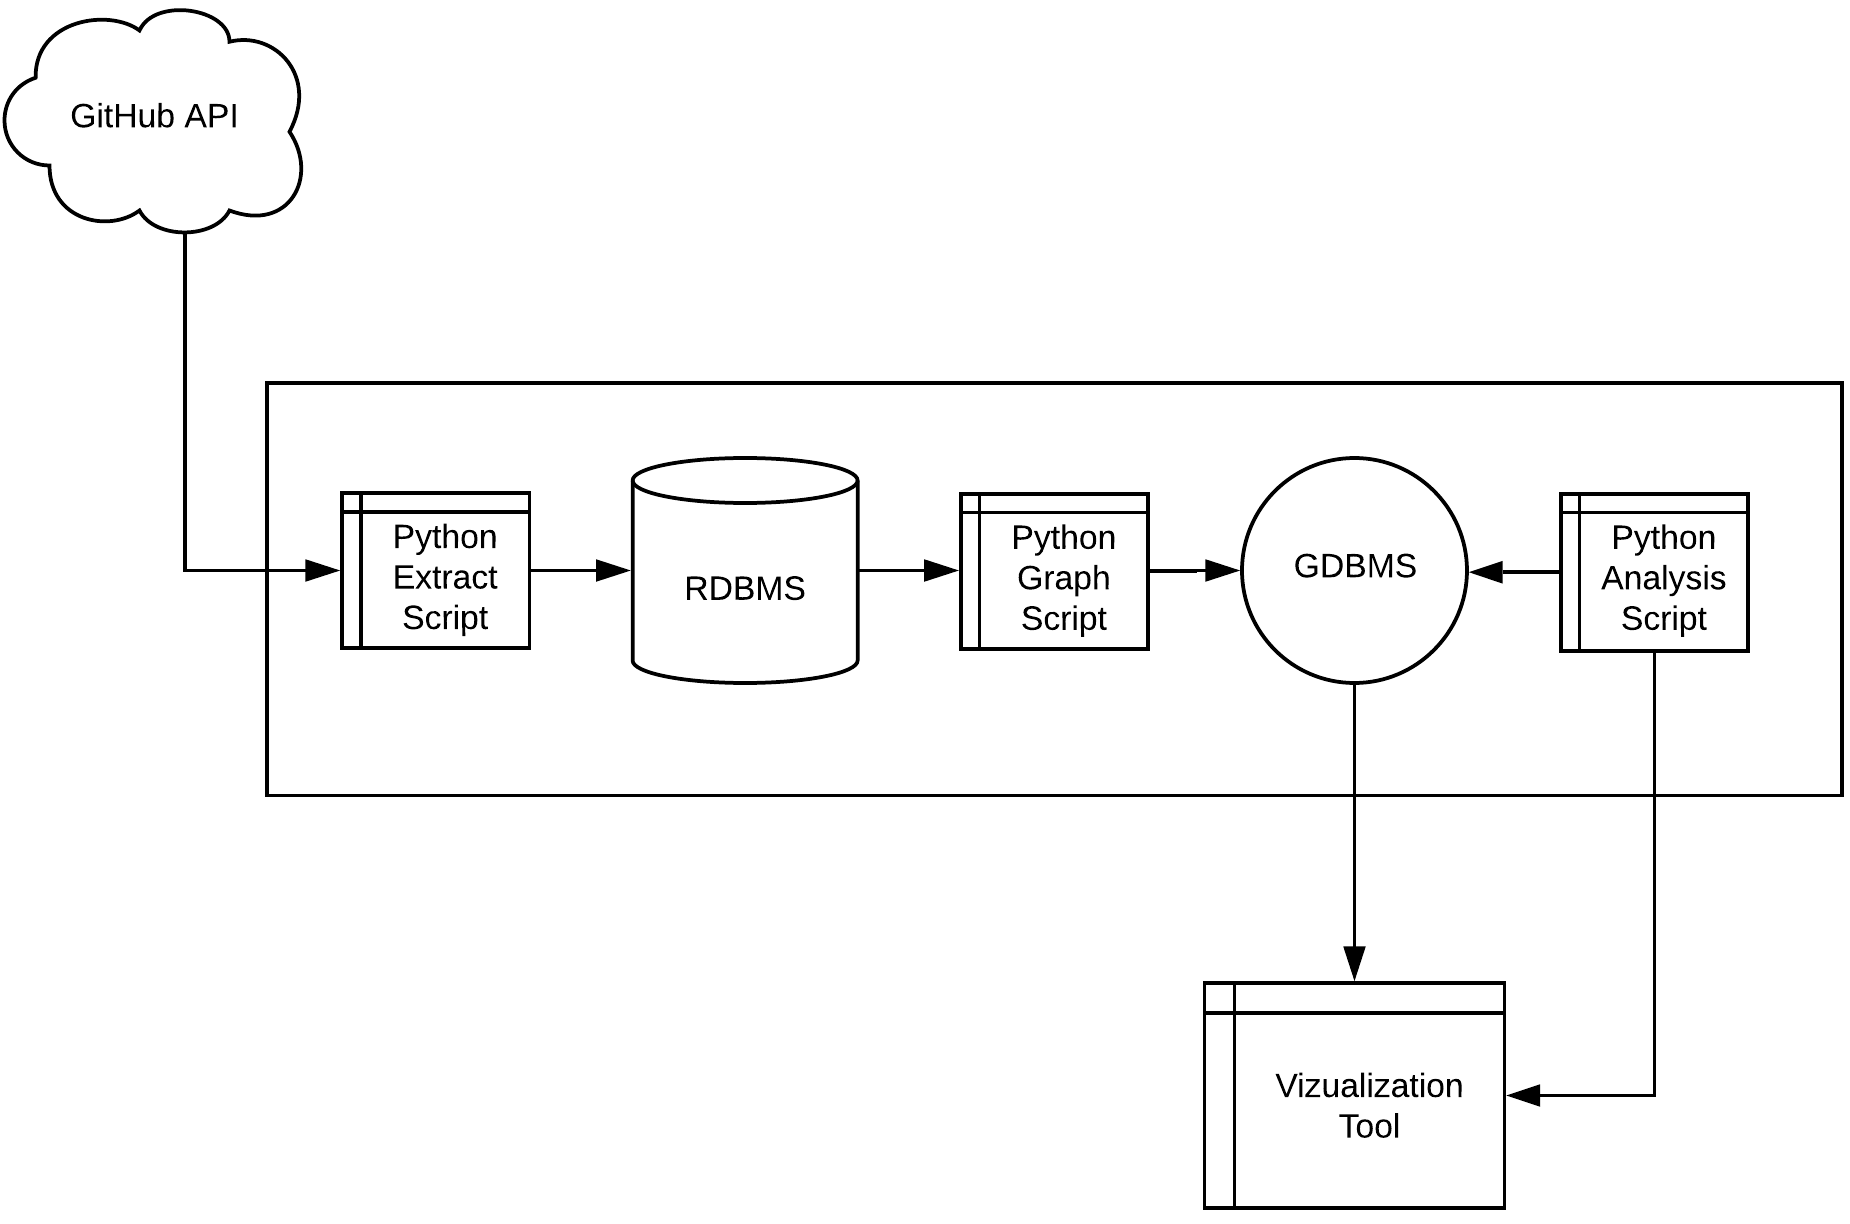
\includegraphics[width=\columnwidth]{processo_extracao}
 \caption{Processo de extração dos dados}\label{fig:processo_extracao}
\end{figure}

Os dados extraídos foram estruturados em um esquema relacional, mais especificamente em uma instância PostgreSQL 10.5. Este passo intermediário ocorreu para que os dados ficassem disponíveis para outras análises, pesquisadores e ferramentas familiarizadas com o modelo relacional. Além disso, esta abordagem permite a extração de diversos metadados que não serão utilizados nas análises preliminares executadas na estrutura baseadas em grafo, ficando disponíveis para consultas posteriores sem degradar o desempenho do modelo em análise. A figura~\ref{fig:mer} mostra o modelo relacional proposto. As entidades \textit{user} são normalizadas entre os diferentes projetos. Ou seja, o usuário é uma entidade única que se relaciona a diferentes projetos, sem duplicação de seu conteúdo. Esta caracterísitca facilita futuras análises de colaboração entre projetos distintos. As \textit{labels} ligadas aos \textit{pullrequests} são utilizadas como descritores semânticos do conteúdo da contribuição, como por exemplo \textit{documentação}, \textit{python} ou \textit{performance}. As contribuições podem ser feitas através de comentários thread de discussão do \textit{pullrequests}, representados pelos \textit{discussioncomments} ou através de comentários no código em revisão, nos \textit{reviewcomments}.

\begin{figure*}[!htbp]
 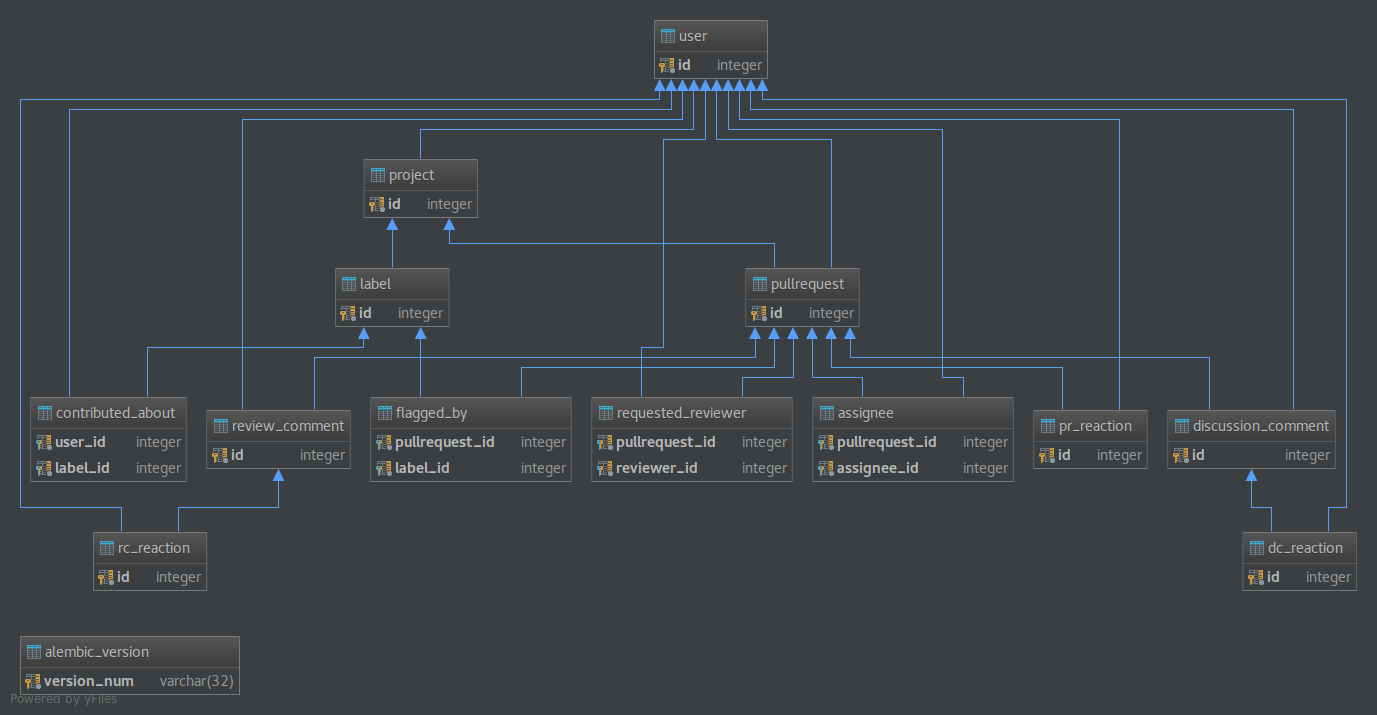
\includegraphics[width=\textwidth]{mer}
 \caption{Modelo Entidade Relacionamento}\label{fig:mer}
\end{figure*}

O algortimo de extração dos dados foi projetado com uma série de cuidados para garantir a integridade e disponibilidade das informações, diante das nuances do repostiório e do domínio de dados. Os principais aspectos observados foram:

\paragraph{Inconsistência nos dados: } Para evitar dados inconsistentes, toda a extração é feita no contexto de uma transaction relacional do SGBD, garantindo que todas as ações sejam executadas (ou canceladas) de forma atômica. As restrições de chave primária também são a primeira linha de defesa para evitar que informações inconsistentes sejam armazenadas (como por exemplo um comentário relacionado a um pullrequest que não existe).

\paragraph{Tratamento das exceções da API: } O repositório de dados pode se comportar de maneira anormal durante a extração dos projetos, por diversos motivos: indisponibilidade dos serviços, lentidão do cliente, problemas de conexão entre outros. Assim foi necessário tratar erros (como 400, 500 e 502) e evitar que o dump seja interrompido. Para isso, as respostas são tratadas, e detectados erros temporários como estes, o request é agendado para se repetir em uma janela de tempo definida.

\paragraph{Ratelimit da API: } A API do GitHub limita o número de requests a 5000/hora. Por isso, é necessário que o cliente controle o número de requests para que não seja bloqueado. Assim, o componente de extração limita o seu número de requests, entrando em espera quando o número se aproxima ao limite imposto.

\paragraph{Unicidade de usuários: } Usuários são entidades espalhadas entre os diferentes projetos. Para possibilitar análises globais e estatísticas realísticas de tamanhos de projetos, é necessário que não haja duplicação entre os usuários. O componente de extração também garante que não hajam usuários duplicados.



\subsection{Aspectos de Reprodutibilidade}

Cada uma das tecnologias apresentadas foram encapsuladas através da tecnologia de virtualização Docker. esta abordagem é uma resposta às iniciativas de reprodutibilidade na ciência, buscando maior transparência, confiabiliade e possibilidade de extensão nos experimentos \cite{freire2012}. Os três componentes (banco de dados relacional, orientado a grafo e os scripts de extração, transformação e carga) foram encapsulados em contâiners distintos, como mostra a figura~\ref{fig:docker-model} Estes foram orquestrados através do docker-compose, que configura os parâmetros e acessos necessários para o funcionamento do sistema sem que o usuário precise realizar nenhuma ação extra.

\begin{figure}[!htbp]
 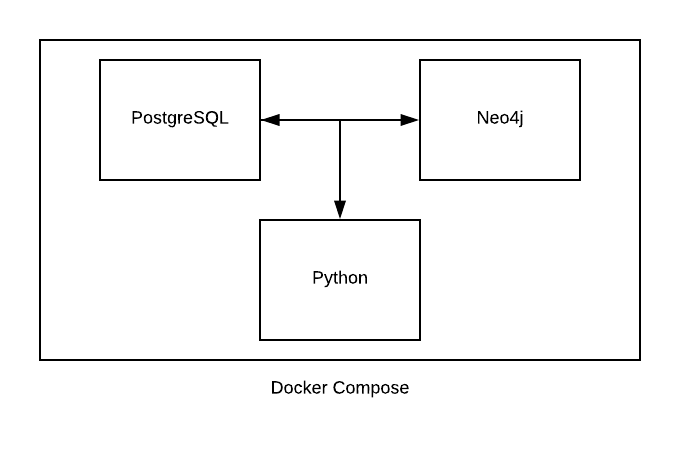
\includegraphics[width=\columnwidth]{docker-model}
 \caption{Modelo de contâiners}\label{fig:docker-model}
\end{figure}


Com um conjunto grande de dependências, tecnologias e minúncias que estão envolvidas neste tipo de experimento, o código fonte e a descrição ainda que detalhada dos dados não são suficiente para alcançar níveis adequados de reprodutibilidade~\cite{ince2012}. Com auxílio dos containers Docker, foi possível criar instâncias executáveis dos experimentos que vão funcionar em diferentes computadores, arquiteturas e situações, sem necessidade de conhecimento técnico por parte do executor das tecnologias utilizadas \cite{boettiger2015}.

De acordo com Sinha et al. \cite{sinha2016}, a maturidade da reprodutibilidade de um experimento científico computacional pode ser medido de acordo o nível dos seguintes aspectos que foram trabalhados em sua disponibilização:

\paragraph{Dados - Evidências Primárias/Secundárias:} Análise da disponibilidade dos dados utilizados para futuros pesquisadores. Pode variar de simplesmente não dispobilizado até a disponibilização íntegra das informações, valendo-se de meios para uma oferta não repudiável e com garantias de integridade e veracidade. Neste trabalho, todos os dados (em suas diferentes agregações) foram disponibilizados para uso futuro\footnote{https://github.com/vschettino/gitrev/blob/groupby\_labels/dumps/complete\_dump2018-08-05.tar.xz}. Além disso os mecanismos de extração são automatizados, permitindo buscar outros projetos ou atualizar os dados dos já utilizados.

\paragraph{Modelo e Parâmetros:} Verificação dos modelos e parâmetros utilizados no experimento. São essenciais para a discussão e reprodução do experimento, além tentativas de otimização. Varia de não disponibilizado até a disponibilização plena com documentação adequada, interface robusta que trate valores fora do domínio (como nulos) e também prática, facilitando os testes com parâmetros e dados distintos. Os modelos de dados e de execução foram detalhados neste trabalho. Além disso, todas as análises são automatizadas e encapusladas através de comandos executáveis dentro de um contâiner Docker.

\paragraph{Código Fonte:} Disponibilidade do código fonte utilizado nas análises. Pode variar de não disponível (proprietário) até open source com direito de extensão e modificação. Neste projeto todo o código fonte é opensource e foi disponibilizado sob a permissiva licença MIT.

\paragraph{Sistema computacional requerido:} Detalhamento das informações de hardware e software necessários, como por exemplo memória, arquitetura, processador, versão e plataforma. O nível ideal é a disponibilização do experimento em ambiente virtualizado em nuvem, em arquitetura que permita tanto a reprodução "as is" quanto extensão e modificação de parâmetros e dados de entrada. Como todo o pipeline deste projeto está disponibilizado na infraestrutura Docker, a única restrição da máquina do pesquisador é ter o Docker instalado.

\subsection{Escolha dos repositórios de dados}

Para avaliar as diferentes propriedades das redes colaborativas propostas, foi necessário definir um conjunto de dados inseridos no contexto de estudo. As principais características buscadas foram:

\paragraph{Repositórios de DDS:} Como a recomendação de revisores têm maior relevância em desenvolvimento global de software, os repositórios escolhidos deveriam ser representantes deste contexto de desenvolvimento.

\paragraph{Acesso aberto: } Os repositórios deveriam estar disponíveis para uso em pesquisa e para futuras reproduções e extensões do estudo. Além disso houve a restrição de estarem no GitHub para acesso via API.

\paragraph{Popularidade e Escala:} Os repostórios deveriam ser razoavelmente conhecidos e possuir um número de contribuidores que justificasse a necessidade de recomendação de revisores. Para isso foram escolhidos projetos integrantes do top-10 "projects with the most reviews" eleitos pelo próprio GitHub\footnote{https://octoverse.github.com/}

A tabela~\ref{tab:repos} ilustra os projetos escolhidos e informações de contexto e tamanho.

\begin{table*}[!h]

\centering
\resizebox{\textwidth}{!}{%
\begin{tabular}{@{}l|l|l|l|l|l|l@{}}
\toprule
\textbf{Nome} & \textbf{Linguagem Principal} & \textbf{Watchers} & \textbf{Stars} & \textbf{Contribuidores} & \textbf{Pull Requests} &  \\ \midrule\hline
Node.js    & JavaScript          & 2.868     & 52.709  & 2.088           & 8.440          &  \\
TensorFlow & C++/Python          & 8.293     & 108.249 & 1.624           & 8.562          &  \\
Kubernetes & Go                  & 2.675     & 40.610  & 1.776           & 41.059         &  \\
Symfony    & PHP                 & 1.297     & 18.381  & 1.692           & 17.475         &  \\ \bottomrule
\end{tabular}%
}
\caption{Descrição dos Respositórios Selecionados}
\label{tab:repos}
\end{table*}

\section{Recomendando Especialistas Entre Projetos}

Especialistas de um projeto podem ser detectados de diversas formas. Analisando a atividade recente, por exemplo, é possível encontrar os desenvolvedores responsáveis pelas principais contribuições. Estas contribuições podem ser revisões, modificações no código, documentação e tradução dos artefatos.

Contudo, o intercâmbio destes especialistas entre projetos distintos é um desafio. Isso porque desenvolvedores podem ser especialistas em determinadas atividades ou tecnologias, e indentificar semelhanças de demandas entre projetos não é trivial. No GitHub, as labels dos pull requests tem como objetivo esta caracterização da modificação que está sendo feita, e por isso ajuda a identificar o tipo de conhecimento que o autor e o revisor demonstram ter influência. Ainda assim, as labels são particulares de cada projeto e podem ser editadas por seus mantenedores, o que reforça o desafio de buscar especialsitas que podem ser úteis em outros projetos.

Para atacar esta barreira, este trabalho propõe o uso de ontologias para alinhar as tags de diferentes projetos. O objetivo é que desenvolvedores conceituados dos projetos alvos do alinhamento tenham uma infraestrutura para documentar e expressar a relação entre as diversas labels dos projetos. Assim, é possível que especialistas encontrados em determinado projeto possam ser recomendados como especialsitas em outros projetos, de acordo com a equivalência das labels envolvidas.

\subsection{Ontologia Proposta}

A ontologia proposta pode ser visualizada na figura~\ref{fig:ontologia}. Apenas duas entidades são criadas, \textit{Project} e \textit{Label}. Entre elas uma Object Property \textit{owns} que denota que determinada label originalmente é originária de determinado projeto.

\begin{figure}[!htbp]
\centering
 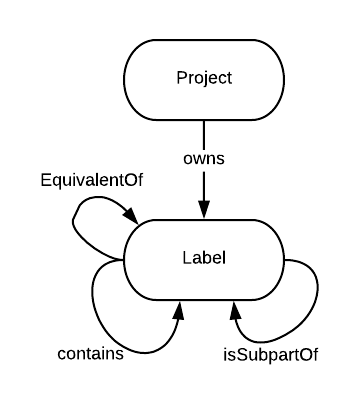
\includegraphics[width=\columnwidth]{ontologia}
 \caption{Visualização da Ontologia Proposta}\label{fig:ontologia}
\end{figure}

As diversas Object Properties que relacionam as \texit{Labels} denotam relacionamento semântico entre elas. Enquanto \textit{contains} siginifica que a \textit{Label} de destino representa parte do conteúdo denotado pela entenidade de origem, \textit{isSubPartOf} traduz o sentido inverso e pode ser inferida pelos \textit{reasoners}. Já \textit{equivalentOf} denota uma correspondência completa entre duas entidades.

Através desta ontologia, é possível expressar os diferentes tipos de equivalência entre labels de projetos distintos. Assim, é possível inferir especialsitas de um projeto que podem contribuir em outro, dentro de suas especialidades já identificadas. Este alinhamento é o principal diferencial da abordagem baseada em ontologias, pois:

\begin{itemize}
  \item Oferece uma interface direta para consulta das \textit{Labels} já alinhadas, sem necessidade de processamento custoso em tempo real.
  \item Permite a utilização de Object Properties para descrever os relacionamentos de forma completa, onde o SGBD se limitaria a relacionamentos triviais como \textit{"de..para"}.
  \item A estrutura é facilmente extensível para criar novos tipos de relacionamento entre as \textit{labels} sem mudanças na estrutura relacional.
\end{itemize}

As próximas subseções detalham como a ontologia proposta pode ser populada e um estudo de caso para averiguar a utilização prática dos métodos descritos.

\subsection{Populando a Ontologia}

Como descrito em seções anteriores, os dados são extraídos dos repositórios distribuidos e consolidados em uma base de dados relacional. Este é o ponto central de onde outras transformações são executadas, como a criação da rede colaborativa. Para popular a ontolgia proposta, é necessário acessar este repositório central. A figura~\ref{fig:workflow_ontologia} mostra o processo de extração para disponibilizar uma interface SPARQL para prover as informações necessárias para os serviços de recomendação.

\begin{figure}[!htbp]
 \centering
 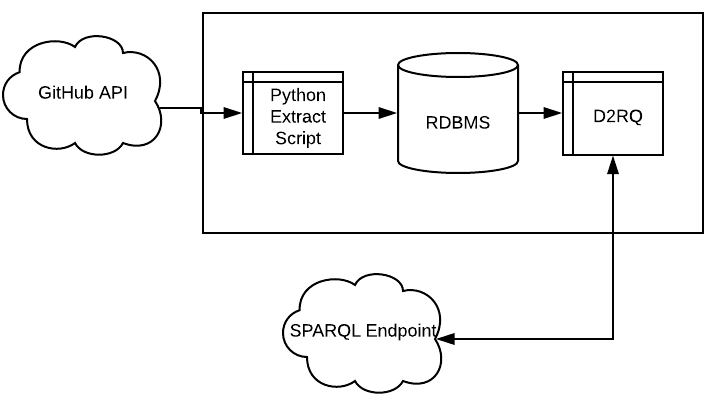
\includegraphics[width=\columnwidth]{workflow_ontologia}
 \caption{Workflow de Extração}\label{fig:workflow_ontologia}
\end{figure}


O script de extração em Python fornece mecanismos para o alinhamento proposto das Labels, para o então fornecimento da interface SPARQL que será utilizada pelos metodos de detecção e recomendação de especialistas entre projetos. Existem diversos métodos para buscar equivalência entre entidades oriundas de repositórios distintos. Algumas são baseadas na semântica ou na sintaxe dos descritores das entidades. Algumas tem como foco o \textit{matching} seguro das informações, evitando ao máximo falsos positivos~\cite{vasilescu2013}. Em outros casos os autores buscam abordagens mais rebuscadas, especialmente para integração de fontes de dados heterogêneas~\cite{silvestri2015}.

Todos os métodos apresentados servem para facilitar o processo de \textit{matching} e evitar o trabalho operacional humano, mas para evitar a existência de falsos positivos, devem ser supervisionados por um especialista, que deve interferir quando achar necessário. Existem outros métodos que podem ser testados no futuro, extendendo o poder de alinhamento automático e auxiliando o processo com mais eficiência. Os principais métodos são:

\begin{itemize}
  \item Direto, buscando \textit{Labels} com descritores idênticos e fornencendo uma relação de \textit{equivalentOf}.
  \item Parcial, buscando proximidade em detrimento de caracteres equivalentes
  \item Radicais, identificando abreviações de labels equivalentes
  \item Relação ``todo-parte'', onde \textit{Labels} são identificadas como ``sublabels'' de outras
\end{itemize}

A tabela~\ref{tab:matching} mostra exemplos de alinhamentos que podem ser identificados automaticamente. Todas as saídas são sugestões de alinhamento para o especialista, que deve aprová-las para utilização posterior dos métodos de detecção e recomendação.

\begin{table}[!h]
  \centering
\begin{tabular}{@{}|l|l|l|@{}}
\hline
Método       & Exemplos de Labels Alinhadas           & Tipo de Relação                 \\ \hline
Direto       & ``python" e ``python"        & \textit{equivalentOf}           \\
Parcial      & ``lib\_src" e ``lib-src"     & \textit{equivalentOf}           \\
Radicais     & ``perf" e ``performance"     & \textit{equivalentOf}           \\
``Todo-Parte" & ``python-crypto" e ``crypto" & \textit{isSubPartOf} \\ \hline
\end{tabular}
\caption{Alinhamento automatizado}\label{tab:matching}
\end{table}

O D2RQ\footnote{http://d2rq.org/} é uma plataforma que provê uma interface de acesso às bases de dados relacionais como triplas RDF, acessíveis através de uma interface que interpreta consultas SPARQL. A conversão entre os modelos é feita nativamente para tipos mais comuns e é baseada na ontologia proposta, e pode ser extendida através do desenvolvimento de classes que implementem o comportamento esperado. A conversão pode ser feita em tempo real ou criando um arquivo TTL (Turtle Triple Language) que solidifica todas as informações necessárias para posterior consulta.

Apesar do poder que as máquinas de inferência possuem, o desemepenho desta abordagem ainda é um fator limitante de sua adoção geral na web semântica \cite{shvaiko2013}. Quando se tratam de grande volumes de dados, os bancos de dados relacionais proveem mais escalabilidade, e por isso abordagens híbridas são aconselhadas~\cite{hepp2008}. Como os projetos opensource encontrados no GitHub possuem centenas de milhares de registros, testes preliminares apontaram pela inviabilidade da inferência através destas tecnologias. Assim, o D2RQ se mostrou como alternativa plausível que permite a especificação de serviços e modelos SPARQL aproveitando o poder da ontologia como linguagem de especificação, permitindo a utilização da infraestrutura relacional que dispõe de maior escalabilidade e desempenho.


\section{Cenário de Utilização}

Para demonstrar o funcionamento da estrutura proposta, foi realizado um estudo de caso com dados reais de um projeto de relevância no GitHub. Como o objetivo deste trabalho é apresentar a abordagem de intermediação de revisores entre projetos distintos, detalhes do método de recomendação utilizado não são apresentados. A abordagem em questão é independente do método de recomendação, uma vez quaisquer especialistas indicados podem ser avaliados de acordo com os tópicos de conhecimento que eles contribuiram, não sendo relevante o método utilizado para sua detecção. Portanto, o foco desta seção é avaliar a eficácia da equivalência entre as \textit{labels} dos projetos distintos. Esta análise pode ser posteriormente utilizada para extender métodos de detecção ou recomendação de revisores.

Buscando por repositórios com quantidades razoáveis de dados, utilizamos o top-5 oficial da plataforma para projetos mais revisados\footnote{https://octoverse.github.com/}, selecionado aquele com mais estrelas. Esta funcionalidade do GitHub pode ser utilizada como medida para o tamanho da comunidade passiva de um projeto\cite{sheoran2014}. Assim, este critério nos levou a escolher o \textbf{Node.js}\footnote{https://github.com/nodejs/node}, uma popular engine JavaScript especialmente utilizada para aplicações \textit{server-side} de alta vazão (I/O).

A organização responsável pelo projeto conta com outros 148 repositórios, a maioria deles bem menores e de alguma forma relacionados ao projeto principal. Para este estudo de caso foram escolhidos repositórios: o \textbf{llnode}\footnote{https://github.com/nodejs/llnode} que mantém um plugin para debug do Node.js e o \textbf{build}\footnote{https://github.com/nodejs/build} que administra o pipeline de deploy e integração contínua da tecnologia.

Para o papel de especialista responsável pelo processo de \textit{matching} foi escolhido um desenvolvedor de software com conhecimento do processo de desenvolvimento dos projetos em questão, bem como as regras de governança e workflow.

Os dados dos três projetos foram extraídos através do processo descrito anteriormente, e disponibilizados na na instância relacional. O script de alinhamento é executado, fornencendo sugestão de equivalência entre as diversas labels. Os resultados são descritos abaixo. Juntos, estes projetos reúnem mais de 200 labels, o que torna o alinhamento completamente manual lento e oneroso. Este aspecto potencializa a importância das técnicas automatizadas para suportar o processo.

Entre o projeto Node.js e o llnode, diversas labels foram alinhadas de maneira direta: ``V8 changes'' e ``feature request'' por exemplo. A segunda é comum a diversos projetos e está mais relacionada ao workflow de desenvolvimento do que efetivamente um tópico de conhecimento, e pode ser negada pelo operador caso ele considere que este não seja um bom fator para recomendação de especialistas para projetos distintos. Utilizando o alinhamento parcial, as tags ``flasky tests'' e ``flasky test'' foram alinhadas. Esta equivalência é relevante pois identificar testes instáveis pode ser uma atribuição compartilhada dos projetos, pois pode estar relacionada à escrita dos testes ou à infraestrutura de execução.

Já entre Node.js e build, houve alinhamento direto entre ``tsc-review'', que indica que o pull request deve ser avaliado pelo Technical Steering Committee do projeto\footnote{https://github.com/nodejs/TSC}. Outros alinhamentos como ``enhancement'' e ``bug'' foram identificados, e provavelmente não servem para detecção de especialistas entre projetos pois são comuns às atividades de software e não necessariamente a um tópico de conhecimento e por isso foram negados pelo operador. Já a comparação por radicais apontou equivalência entre as labels ``install'' e ``installer'', que parecem ter funções parecidas nos projetos mas foram grafadas de forma distinta. Neste aspecto o alinhamento parece relevante, pois os principais revisores em cada uma destas labels são os mesmos em cada um dos projetos.

Com este estudo de caso foi possível observar que algumas equivalências automatizadas competem a tópicos muito generalistas, onde um especialista de determinado projeto não parece ter competência explícita para o ser em outro. Contudo, diversas equivalências parecem ser relevantes para os projetos selecionados, e por isso podem expressar relacionamentos que apoiam o processo de alinhamento manual. Estudos de caso posteriores podem ajudar a investigar se os especialistas têm performance equiparável quando contribuindo em outros projetos.

\section{Conclusão}\label{cha:conclusao}

O \textit{code review} é uma prática estabelecida com efeitos conhecidos e confirmados por vários autores através dos anos. Desde o processo tradicional que nasceu nos anos 70" baseado em um workflow rígido, a técnica se desenvolveu constantemente para o modelo leve e ágil que valoriza mais a troca de conhecimento e a relação entre pessoas.

Estudos recentes mostram o impacto da escolha do revisor correto na eficiência e impacto do processo na qualidade do código e na detecção precoce de defeitos. Isso fez com que diversos autores propossem métodos para recomendar revisores adequados, dado o contexto e o conteúdo de umaa revisão. Os desafios do desenvolvimento global de software potencializam a necessidade desta recomendação, visto a quantidade de informações que influenciam na capacidade do revisor e a dificuldade de agregá-las de forma manual, levando a escolhas tardias ou fundamentalmente ruins.

Trabalhos mais recentes apresentam propostas e métodos de avaliação baseados em informações de colaboração, como atividade, eficiência de revisões passadas e capacidade de interação. Estes resultados motivaram a proposta de novos métodos de recomendação baseados em redes colaborativas e voltados para o desenvolvimento global de software, com suas peculiaridades.

Para expansão dos métodos já avaliados, especialistas podem ser recomendados para projetos distintos de suas contribuições originais. Para isso, este trabalho propõe a utilização de ontologias para alinhamento dos tópicos de semânticos internos dos repositórios, de forma a inferir que se um desenvolvedor domina determinado conhecimento de um projeto, poderá auxiliar em outro projeto com demandas equivalentes. Para testar esta hipótese, foi descrito um cenário de uso com o alinhamento de projetos relevantes da comunidade OpenSource. Foram identificadas diversas equivalências, algumas relevantes e outras que podem ser negadas pelo o operador do processo, um especialista realiza a curadoria do alinhamento e julga as sugestões geradas automaticamente.

A abordagem proposta pode ser utilizada para extender métodos de recomendação de revisores de código, levando resultados relevantes para projetos distintos, baseada nas equivalências dos tópicos de conhecimento que podem existir entre projetos correlatos. Utilizando as \textit{labels} que categorizam os \textit{pullrequests} dos projetos, é possível identificar que potenciais revisores em determinadas linguagens, bibliotecas e tecnologias podem contribuir em outros projetos que compartilhem das mesmas necessidades.

Como trabalhos futuros, existem diversas aplicações de ontologia nos métodos propostos. É possível sua utilização para integração e alinhamento dos dados de diferentes bases que contém informações sobre desenvolvedores e sua reputação, como o StackOverflow e ferramentas como o Twitter. Além disso, testes aprofundados e avaliação dos métodos de recomendação conhecidos podem apontar novas aplicações de ontologia com o objetivo de melhorar a qualidade das saídas e a predição de revisores cada vez mais adequados. Para aumentar a eficácia do processo de equivalência dos tópicos semânticos, pretendemos utilizar um Tesauro, como o WordNet\footnote{https://wordnet.princeton.edu/}. Através dos sinônimos cognitivos (\textit{synsets}) pode ser possível encontrar equivalências mais adequadas e sem embasamento direto na sintaxe dos léxicos. Por fim, queremos realizar avaliações aprofundadas da efetividade que desenvolvedores indicados entre projetos distintos no processo de code review.

\bibliographystyle{ACM-Reference-Format}
\bibliography{../bibrefs/refs}

\end{document}
